% numberline
\documentclass[preview,12pt]{standalone}
\usepackage{tikz}
\usetikzlibrary{positioning, arrows.meta, bending}
\usepackage{ulem}
\usepackage[a4paper, portrait, margin=1cm]{geometry}

\def\jumpheight{10}
\def\qgap{\raisebox{-1pt}{\dotuline{\phantom{X}}}}

% modify values for number lines
\def\minval{-10}
\def\midval{0}
\def\maxval{10}
\def\startval{-4}
\def\midstep{1} % Second step at least 2 units away
\def\endval{7}

% values for display
\def\startvaltxt{\startval}
\def\midsteptxt{\midstep}
\def\endvaltxt{\endval}
\def\changevaltxt{\the\numexpr\endval-\startval\relax}
\def\firstjumptxt{\the\numexpr\midstep-\startval\relax}
\def\secondjumptxt{\the\numexpr\endval-\midstep\relax}
\def\equtxt{\the\numexpr\startval\relax + \the\numexpr\firstjumptxt\relax + \the\numexpr\secondjumptxt\relax = \the\numexpr\endval\relax}

\begin{document}
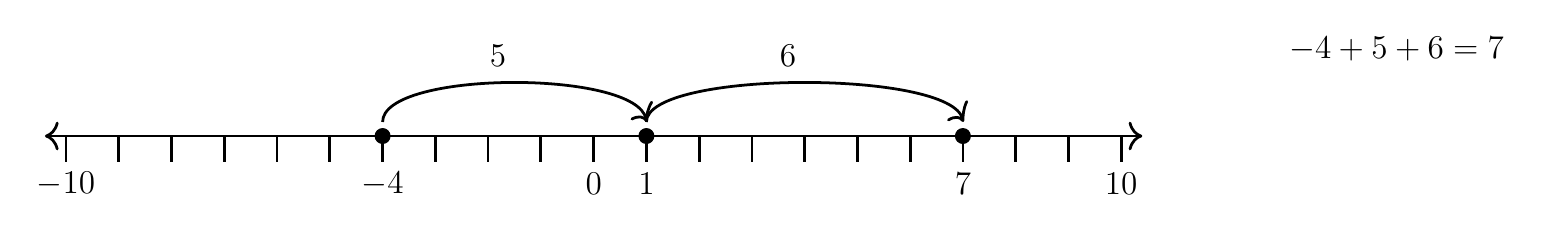
\begin{tikzpicture}[scale=0.67]
    % axis
    \draw[{To[scale=1.3]}-{To[scale=1.3]}, line width=1pt] (\minval-0.4, 0) -- (\maxval+0.4, 0);

    % tick marks
    \pgfmathtruncatemacro{\nextmin}{\minval+1}
    \foreach \x in {\minval,\nextmin,...,\maxval}
        \draw[shift={(\x,0)},color=black, line width=1pt] (0pt,-14pt) -- (0pt,0pt);

    % numbers along each axis
    \foreach \x in {\minval,\midval,\maxval} {
        \draw[shift={(\x,-0.8)},color=black] node[font=\large,text height=12pt] {$\x$};
    }

    % Start, Midstep, and End value labels
    \draw[shift={(\startval,-0.8)},color=black] node[font=\large,text height=12pt] {$\startvaltxt$};
    \draw[shift={(\midstep,-0.8)},color=black] node[font=\large,text height=12pt] {$\midsteptxt$};
    \draw[shift={(\endval,-0.8)},color=black] node[font=\large,text height=12pt] {$\endvaltxt$};

    % dots
    \filldraw[black] (\startval,0) circle (4pt) node[above,yshift=-2pt] (a) {};
    \filldraw[black] (\midstep,0) circle (4pt) node[above,yshift=-2pt] (m) {};
    \filldraw[black] (\endval,0) circle (4pt) node[above,yshift=-2pt] (b) {};

    % first arrow
    \draw[-{To[scale=1.3, bend]},line width=1pt, color=black] (a.north)
        .. controls  +(north:\jumpheight mm) and +(north:\jumpheight mm) ..
        node[above=2pt,xshift=-6pt,font=\large,text height=10pt] {$\firstjumptxt$} (m.north);

    % second arrow
    \draw[-{To[scale=1.3, bend]},line width=1pt, color=black] (m.north)
        .. controls  +(north:\jumpheight mm) and +(north:\jumpheight mm) ..
        node[above=2pt,xshift=-6pt,font=\large,text height=10pt] {$\secondjumptxt$} (b.north);

    % equation at right end
    \node [font=\large, anchor=west] at (\maxval+3,1.65){$\equtxt$};
\end{tikzpicture}
\end{document}
